\documentclass{amsart}
\usepackage[margin=1in]{geometry}
\usepackage[english]{babel}
\usepackage[utf8]{inputenc}
\usepackage{subcaption}
\usepackage{amsmath}
\usepackage{amssymb}
\usepackage{amsfonts}
\usepackage{amsthm}
\usepackage{mathrsfs}
\usepackage[all]{xy}
\usepackage[pdftex]{graphicx}
\usepackage{color}
\usepackage{cite}
\usepackage{url}
\usepackage{indentfirst}
\usepackage[labelfont=bf,labelsep=period,justification=raggedright]{caption}
\usepackage{hyperref}
\usepackage{tikz}
\usetikzlibrary{calc}
\usepackage{multicol}
\PassOptionsToPackage{dvipsnames,svgnames}{xcolor}
\usepackage{textcomp}
\usepackage{bbm}
\usepackage[ruled, noend]{algorithm2e}

\graphicspath{{../UI/public/figures/}{./}}

\newtheorem{theorem}{Theorem}
\newtheorem*{theorem*}{Theorem}
\newtheorem{lemma}{Lemma}
\newtheorem{claim}{Claim}
\newtheorem{example}{Example}
\newtheorem{define}{Definition}
\newtheorem{problem}{Problem}
\newtheorem{proposition}{Proposition}
\newtheorem{conjecture}{Conjecture}
\newtheorem{exercise}{Exercise}[subsubsection]
\newtheorem{corollary}{Corollary}

\setlength{\parindent}{0cm}

\title{Iterative Root-Finding Methods and the Polynomial Factorization Procedure}
\author{Kartikesh Mishra}
\date{January 2025}

\begin{document}

\maketitle

\begin{abstract}
This paper implements and analyzes Newton's method, the secant method, and the bisection method to estimate real roots of univariate polynomials. We compare convergence rates, basins of attraction, and failure modes through theoretical and computational analysis. Newton's method achieves quadratic convergence ($q = 2$) for simple roots and linear convergence ($q = 1 - 1/k$) for roots of multiplicity $k$, whereas the bisection method guarantees linear convergence ($q = 1$) across any sign-changing bracket, and the secant method achieves superlinear convergence of order equal to the golden ratio ($\phi = \frac{1+\sqrt{5}}{2} \approx 1.618$). Finally, by combining Cauchy root bounds, critical-point partitioning, and inflection-guided Newton initialization, we introduce the \textbf{Polynomial Factorization Procedure (PFP)}---a recursive algorithm that deterministically isolates and approximates all real roots of any polynomial along with their exact multiplicities.
\end{abstract}

\section{Introduction}\label{sec_intro}

A recurring problem in mathematics and scientific computing is to find the roots of polynomials. Computer software systems usually look for roots numerically rather than symbolically, through iterative estimation methods that converge closer and closer to the actual root with each step. We can compare root-finding methods by how fast they converge and by their failure cases; often, choosing the appropriate method involves a trade-off between fast convergence and robustness (having minimal failure cases).

In this paper, we investigate three foundational iterative root-finding methods for polynomials in one variable: Newton's method, the secant method, and the bisection method. For each of these methods, we analyze the parameters for initial guesses that may cause them to fail to converge, the relation between input parameters and the roots they converge to, and when they converge, their order of convergence.

First, we begin with a simple example to demonstrate the three methods and intuitively describe what each seeks to accomplish. For consistency, we use the same polynomial across all three initial examples:
\[
    f(x) = \frac{1}{8}x^2 - \frac{1}{2}.
\]
The positive root we seek to approximate through these algorithms, which we denote $\alpha$, equals $2$.

\subsection{Newton's Method}
Newton's method accepts an initial guess, $x_0$. Then, it evaluates the function $f(x_0)$ and its derivative $f'(x_0)$, and uses these values to draw a tangent line to the curve at the point $(x_0, f(x_0))$. The algorithm's subsequent guess, $x_n$ (for integers $n>0$), is the $x$-coordinate where this tangent line crosses the $x$-axis. We repeat the process until $|f(x_n)|$ is sufficiently close to $0$. Figure~\ref{fig:newton_ex1} and Table~\ref{tab:newtons_method} show the iterations of Newton's method on our example polynomial, terminating when the error term $e_n = x_n - \alpha$ is less than $10^{-5}$ in absolute value.

\begin{figure}[ht]
    \centering
    \begin{minipage}{0.48\textwidth}
        \centering
        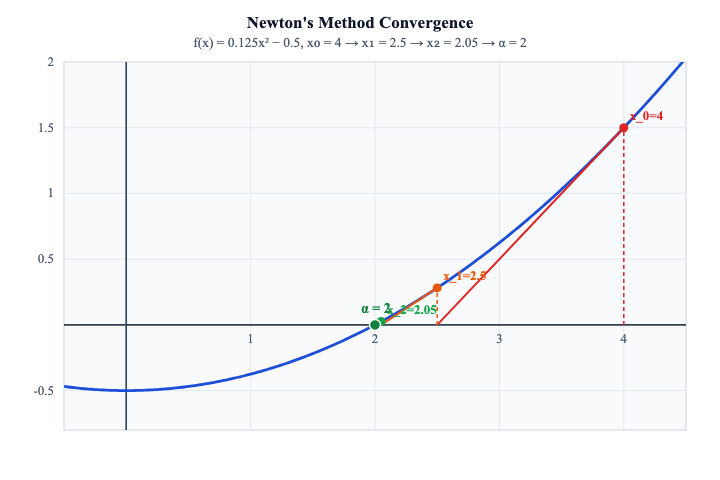
\includegraphics[width=\textwidth]{NewtonEx1.png}
        \caption{Example of Successful Convergence of Newton's Method}
        \label{fig:newton_ex1}
    \end{minipage}\hfill
    \begin{minipage}{0.48\textwidth}
        \centering
        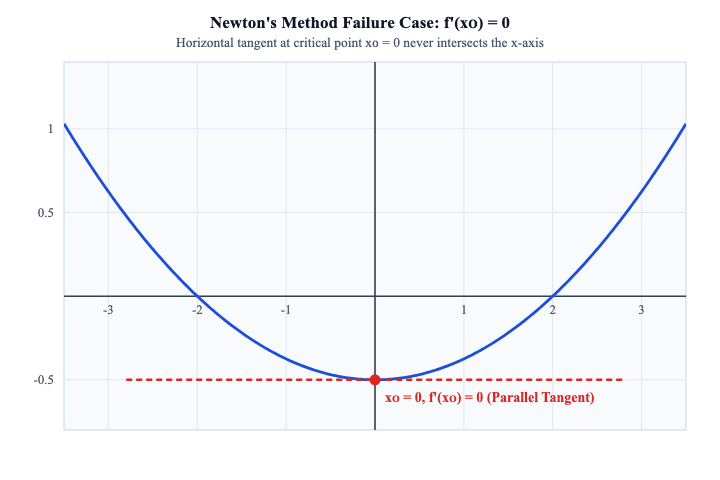
\includegraphics[width=\textwidth]{NewtonFailure1.png}
        \caption{Example of Newton Method Failure: $f'(x_0) = 0$}
        \label{fig:newton_failure1}
    \end{minipage}
\end{figure}

\begin{table}[ht]
\centering
\caption{Newton's Method Iterations for $f(x) = \frac{1}{8}x^2 - \frac{1}{2}$}
\label{tab:newtons_method}
\begin{tabular}{|c|c|c|c|c|}
\hline
Step & $x_n$ & $\alpha$ & $e_n$ & $f(x_n)$ \\
\hline
0 & 4.000000 & 2 & 2.000000 & 1.500000 \\
\hline
1 & 2.500000 & 2 & 0.500000 & 0.281250 \\
\hline
2 & 2.050000 & 2 & 0.050000 & 0.025312 \\
\hline
3 & 2.000610 & 2 & 0.000610 & 0.000305 \\
\hline
4 & 2.000000 & 2 & 0.000000 & 0.000000 \\
\hline
\end{tabular}
\end{table}

We immediately notice that, since Newton's method requires evaluating $f'(x_n)$ at every step in order to construct the tangent line, the method fails if at any point $f'(x_n) = 0$. Visually, $f'(x_n) = 0$ causes the tangent line to run parallel to the $x$-axis, as illustrated in Figure~\ref{fig:newton_failure1}.

\subsection{Secant Method}
The Secant method uses a sequence of secant lines to approximate a root of a function without computing analytical derivatives. Using two initial guesses, $x_0$ and $x_1$, the method evaluates $f(x_{n-1})$ and $f(x_n)$ at each step and computes the $x$-intercept of the secant line passing through $(x_{n-1}, f(x_{n-1}))$ and $(x_n, f(x_n))$. Figure~\ref{fig:secant_ex1} and Table~\ref{tab:secants_method} display the iterations of the Secant method applied to $f(x) = \frac{1}{8}x^2 - \frac{1}{2}$.

\begin{figure}[ht]
    \centering
    \begin{minipage}{0.48\textwidth}
        \centering
        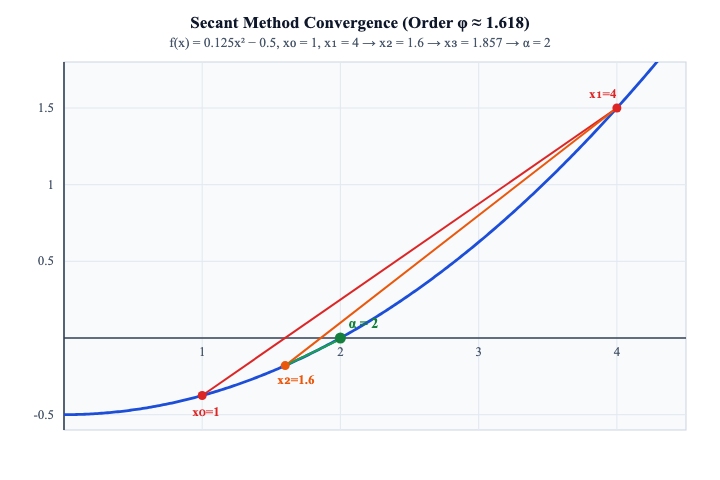
\includegraphics[width=\textwidth]{SecantEx1.png}
        \caption{Example of Successful Convergence of Secant Method}
        \label{fig:secant_ex1}
    \end{minipage}\hfill
    \begin{minipage}{0.48\textwidth}
        \centering
        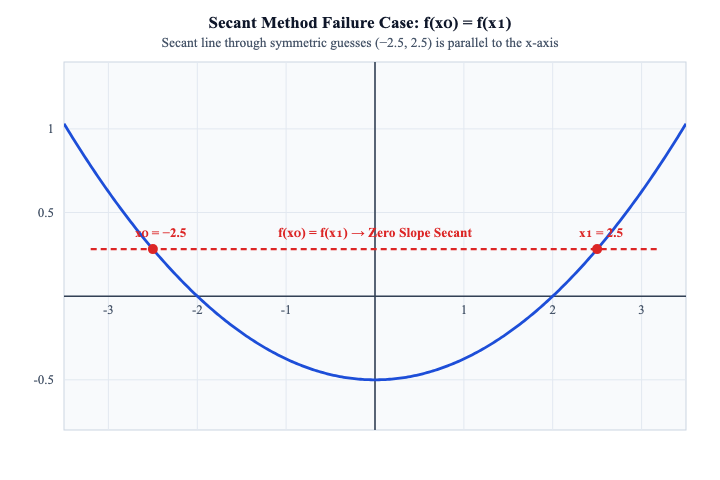
\includegraphics[width=\textwidth]{SecantFailure1.png}
        \caption{Example of Secant Method Failure: $f(x_0) = f(x_1)$}
        \label{fig:secant_failure1}
    \end{minipage}
\end{figure}

\begin{table}[ht]
\centering
\caption{Secant Method Iterations for $f(x) = \frac{1}{8}x^2 - \frac{1}{2}$}
\label{tab:secants_method}
\begin{tabular}{|c|c|c|c|c|c|}
\hline
Step & $x_n$ & $x_{n+1}$ & $\alpha$ & $e_n$ & $f(x_n)$ \\
\hline
0 & 1.000000 & 4.000000 & 2 & -1.000000 & -0.375000 \\
\hline
1 & 4.000000 & 1.600000 & 2 & 2.000000 & 1.500000 \\
\hline
2 & 1.600000 & 1.857143 & 2 & -0.400000 & -0.180000 \\
\hline
3 & 1.857143 & 2.016529 & 2 & -0.142857 & -0.068878 \\
\hline
4 & 2.016529 & 1.999390 & 2 & 0.016529 & 0.008299 \\
\hline
5 & 1.999390 & 1.999997 & 2 & -0.000610 & -0.000305 \\
\hline
6 & 1.999997 & 2.000000 & 2 & -0.000003 & -0.000001 \\
\hline
\end{tabular}
\end{table}

Similarly to Newton's method, the secant method fails when the secant line connecting $x_{n-1}$ and $x_n$ fails to cross the $x$-axis, which occurs whenever $f(x_{n-1}) = f(x_n)$ (Figure~\ref{fig:secant_failure1}).

\subsection{Bisection Method}
The Bisection method iteratively narrows down an interval $[l_n, r_n]$ where a root must lie, starting from an initial bracket $[l_0, r_0]$ satisfying $f(l_0)\cdot f(r_0) < 0$. At each step, the midpoint $x_n = \frac{l_n + r_n}{2}$ is evaluated and replaces whichever endpoint shares its sign. Figure~\ref{fig:bisection_ex1} and Table~\ref{tab:bisection_method} illustrate the Bisection method on $f(x) = \frac{1}{8}x^2 - \frac{1}{2}$ over $[1, 4]$.

\begin{figure}[ht]
    \centering
    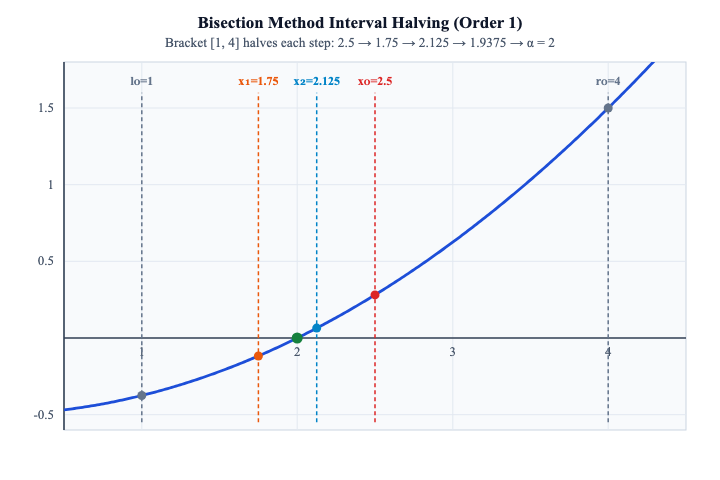
\includegraphics[width=0.58\textwidth]{BisectionEx1.png}
    \caption{Bisection Method Iterations with Initial Interval $[1,4]$}
    \label{fig:bisection_ex1}
\end{figure}

\begin{table}[ht]
\centering
\caption{Bisection Method Iterations for $f(x) = \frac{1}{8}x^2 - \frac{1}{2}$}
\label{tab:bisection_method}
\begin{tabular}{|c|c|c|c|c|c|}
\hline
Step & $l_n$ & $r_n$ & $\alpha$ & $e_n$ & $f(x_n)$ \\
\hline
0 & 1.000000 & 4.000000 & 2 & 0.500000 & 0.281250 \\
\hline
1 & 1.000000 & 2.500000 & 2 & -0.250000 & -0.117188 \\
\hline
2 & 1.750000 & 2.500000 & 2 & 0.125000 & 0.064453 \\
\hline
3 & 1.750000 & 2.125000 & 2 & -0.062500 & -0.030762 \\
\hline
4 & 1.937500 & 2.125000 & 2 & 0.031250 & 0.015747 \\
\hline
5 & 1.937500 & 2.031250 & 2 & -0.015625 & -0.007782 \\
\hline
6 & 1.984375 & 2.031250 & 2 & 0.007812 & 0.003914 \\
\hline
7 & 1.984375 & 2.007812 & 2 & -0.003906 & -0.001951 \\
\hline
8 & 1.996094 & 2.007812 & 2 & 0.001953 & 0.000977 \\
\hline
9 & 1.996094 & 2.001953 & 2 & -0.000977 & -0.000488 \\
\hline
10 & 1.999023 & 2.001953 & 2 & 0.000488 & 0.000244 \\
\hline
11 & 1.999023 & 2.000488 & 2 & -0.000244 & -0.000122 \\
\hline
12 & 1.999756 & 2.000488 & 2 & 0.000122 & 0.000061 \\
\hline
13 & 1.999756 & 2.000122 & 2 & -0.000061 & -0.000031 \\
\hline
14 & 1.999939 & 2.000122 & 2 & 0.000031 & 0.000015 \\
\hline
15 & 1.999939 & 2.000031 & 2 & -0.000015 & -0.000008 \\
\hline
16 & 1.999985 & 2.000031 & 2 & 0.000008 & 0.000004 \\
\hline
\end{tabular}
\end{table}

Even on this single quadratic example $f(x) = \frac{1}{8}x^2 - \frac{1}{2}$, a striking disparity in convergence speed emerges: Newton's method reaches six-decimal accuracy in just $4$ iterations (Table~\ref{tab:newtons_method}), the secant method requires $6$ iterations (Table~\ref{tab:secants_method}), and the bisection method requires $16$ iterations (Table~\ref{tab:bisection_method}). Conversely, the faster methods exhibit sharper failure modes when initialized poorly—Newton's method fails completely if $f'(x_n) = 0$, and the secant method fails if $f(x_n) = f(x_{n-1})$—whereas the bisection method is guaranteed to converge whenever a sign-changing bracket $[l_0, r_0]$ is provided, failing only when all roots have even multiplicity. These trade-offs are summarized in the following comparison:

\begin{center}
\begin{tabular}{|c|c|c|c|} \hline
\textbf{Method} & \textbf{Order of Convergence} & \textbf{Robustness} & \textbf{Derivative Requirement} \\ \hline
Newton & $2$ (simple roots), $1$ (multiple) & Sensitive to $x_0$, cycles & Requires $f'(x)$ \\ \hline 
Secant & $\phi = \frac{1+\sqrt{5}}{2} \approx 1.618$ & Fails if $f(x_n)=f(x_{n-1})$ & Derivative-free \\ \hline 
Bisection & $1$ (linear) & Guaranteed on sign change & Derivative-free \\ \hline
PFP (Ours) & $2$ (on isolated brackets) & Finds all real roots + multiplicities & Uses $f'(x)$ and $f''(x)$ \\ \hline
\end{tabular}
\end{center}

To rigorously measure and compare the rate at which each iterative method approaches a root $\alpha$, we formally define the \textit{order of convergence}.

\begin{define}[Order of Convergence]
A sequence $x_n$ that converges to a root $\alpha$ has \textbf{order of convergence} $q$ if
\[
    \lim_{n\to\infty} \frac{|x_{n+1}-\alpha|}{|x_n-\alpha|^q} = \mu
\]
for some positive constant $\mu$, called the asymptotic error constant.
\end{define}

Intuitively, an estimate that converges with order $q = 1$ (linear convergence) gains a constant number of accurate digits per iteration, whereas an estimate that converges with order $q = 2$ (quadratic convergence) roughly doubles the number of significant digits at every step.

Beyond their local convergence rates, a fundamental limitation shared by all three classical methods is that each solves for only a single local root and provides no global information on how many real roots a polynomial possesses, or whether a polynomial has any real roots at all. To overcome both the initial-guess sensitivity of Newton's method and the single-root limitation of all three algorithms, the remainder of this paper develops a global structural theory of polynomials and culminates in the \textbf{Polynomial Factorization Procedure (PFP)} in Section~\ref{sec_poly}.

\end{document}
